%
% Hierarchical Framework Chapter
% Jason Brownlee
%

\chapter{Hierarchical Frameworks}
\label{chap:framework}

%
% Overview
% Provides an overview of the chapter and its structure, and a description of what is intended to be achieved by providing this documentation. A description of why and how this chapter follows on from the previous chapter
%
\section{Chapter Overview}
\label{sec:framework:overview}
% previous
The previous chapters outlined three distinct perspectives on the clonal selection adaptive strategy phrased as a \emph{Cellular} (Chapter \ref{chap:cells}), \emph{Tissue} (Chapter \ref{chap:tissues}), and \emph{Host} (Chapter \ref{chap:hosts}) Clonal Selection Paradigms. 
% this chapter
This chapter considers all three paradigms together and aggregates the models, algorithms, and problems into a series of hierarchical frameworks. 
% sections
Specifically, Section~\ref{sec:framework:hcsf} integrates the clonal selection models and algorithms,  Section~\ref{sec:framework:haef} integrates the antigenic exposure paradigm, and Section~\ref{sec:framework:ihcsf} combines the clonal selection and antigenic exposure frameworks into an integrated hierarchical clonal selection framework.
% explanatory and predictive
The frameworks provide both explanatory tools for the design decisions and limitations of the investigated algorithms, as well as predictive power as to organisations and configurations that may reveal new and interesting findings regarding the underlying adaptive strategy. 
% broader and generality
Finally, Section~\ref{sec:framework:ihcsf:applicability} considers the methodology behind the framework, the application of the framework to the broader field of AIS, and the general applicability of the methodology to related computational intelligence sub-fields.

%
% Clonal Selection Framework
%
\section{Clonal Selection Framework}
\label{sec:framework:hcsf}

%
% Paradigms
%
\subsection{Paradigms}
\label{sec:framework:hcsf:paradigms}
% natural relationship
The three paradigms considered in this work provide tangible contributions to the field of Artificial Immune Systems, including: (1) varied perspectives of clonal selection as an adaptive strategy, and (2) algorithms within those perspectives inspired by the computational and information processing attributes of the clonal selection theory. The perspectives of clonal selection were selected to promote a natural hierarchical relationship where the tier that followed encompassed the concerns of the tier that proceeded. 
% this section
This section considers the integration of the clonal selection models and algorithms from the \emph{Cellular}, \emph{Tissue}, and \emph{Host} Clonal Selection Paradigms into a \emph{Hierarchical Clonal Selection Framework (HCSF)}. 
% integration
The focus of this framework is on the explicit integration of the information processing concerns of the each of the paradigms as abstractions of the clonal selection theory at difference scales and scopes of the acquired immune system.
% what we get
This integration facilitates (1) inter-paradigm contrast and comparison, and (2) analysis and reasoning on the framework providing both explanatory and predictive capabilities regarding abstractions of the clonal selection theory.
% perspective of this framework
The focus of the framework is on the systems side of the system-environment relationship, and as such the concerns of the antigenic exposure paradigm may be compressed to a generic cross-paradigm antigen exposure problem (see Figure~\ref{fig:framework:hcsf:interpretation:expanded-flat}). This simplification of the environment directs focus on the elaboration, and inter-relationships on the systems. 

\begin{figure}[htp]
	\centering
	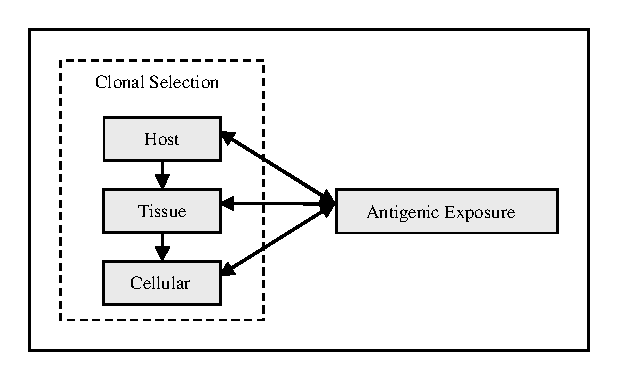
\includegraphics[scale=0.85]{Framework/framework-integration-expanded-flat}
	\caption{Depiction of the focus on systems and the compression of the environment in the Hierarchical Clonal Selection Framework (HCSF).}
	\label{fig:framework:hcsf:interpretation:expanded-flat}
\end{figure}

%
% Comparison
%
\subsection{Comparison}
\label{sec:framework:hcsf:comparison}
% the formalism as a tool
This section directly compares the three paradigms beyond the obvious and superficial concerns of the perspectives and the algorithms within. Toward this end, the adaptive systems formalism from Section~\ref{subsec:cs:adaptive} is used as a basis to motivate the comparison. This formalism was selected because it explicitly provides a tool for considering the similarities and differences between adaptive systems (paradigms), and importantly between strategies (algorithms within a paradigm).
% primary objects
The primary objects of the adaptive systems formalism provide a conventional perspective on the components of an adaptive system (see Table~\ref{tab:adaptsys:primary}). From this high-level perspective the subtleties of the three paradigms are lost and one may consider the generalities of the clonal selection adaptive strategy, specifically: the antigenic environment ($e$), the clonal selection strategy in cells ($s$), and the affinity of cells to antigen ($U$). This consideration compresses the hierarchy to the essential concerns of the adaptive strategy (for example see Figure~\ref{fig:framework:hcsf:interpretation:flat-flat}). This is an important perspective, as (1) it highlights the important primitives required in all so-called `Clonal Selection Algorithms', (2) provides a context for comparing the general approach to other adaptive strategies such as genetic adaptive plans (the basis of genetic algorithms), and (3) provides a context for relating and integrating the general approach to other Artificial Immune System approaches (for example clonal selection as a sub-strategy in Negative Selection and Immune Network algorithms).

\begin{figure}[htp]
	\centering
	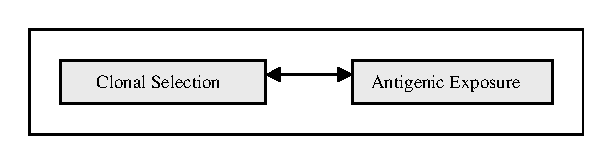
\includegraphics[scale=0.85]{Framework/framework-integration-flat-flat}
	\caption{Depiction of the compression of both the system and the environment when the HCSF is compressed to the primary objects of the adaptive system formalism.}
	\label{fig:framework:hcsf:interpretation:flat-flat}
\end{figure}

% secondary objects
The secondary objects promote the consideration of the subtler details of an adaptive system, providing the detail of the formalism (see Table~\ref{tab:adaptsys:secondary}). Table~\ref{tab:framework:hcsf:secondaryobjects} provides an interpretation of the three paradigms in the context of the secondary objects of the formalism specifically motivated by Holland's fundamental questions listed in Table~\ref{tab:adaptsys:questions}.

\begin{table}[htp]
	\centering\small
		\begin{tabularx}{\textwidth}{lXXX}
		\toprule
		 & \textbf{Cellular}  & \textbf{Tissue}  & \textbf{Host} \\ 
		\toprule
		$A$ & Cell & Tissue & Host \\ 
		\midrule
		$E$ & Antigen & Infections & Habitats \\ 
		\midrule
		$O$ & Interaction of cells & Movement and capacity of cells & Movement of antigen and cells \\ 
		\midrule
		$S$ & Single repertoire & Discrete tissue and constrained connectivity & Discrete Hosts \\ 
		\midrule
		$X$ & Composition and capability & Acquisition and anticipation of need & Acquisition and anticipation of need \\ 
		\midrule
		$I$ & Selection & Spatial-temporal selection & Spatial-temporal selection \\ 
		\midrule
		$M$ & Proportional resource allocation & Spatial organisation & Spatial organisation \\ 
		\bottomrule
		\end{tabularx}
	\caption{Mapping of the cellular, tissue, and host clonal selection perspectives onto the secondary objects of the adaptive systems formalism.}
	\label{tab:framework:hcsf:secondaryobjects}
\end{table}

% structures and environments
The naming convention adopted for the three tiers highlights the structures or units under adaptation within each tier. This naming convention is mirrored in the areas of the environment to which each structure is adapting. 
% subsumption structures
The consideration of the adaptive structures highlights the already apparent subsumption of cellular concerns by the tissue tier, and the tissue concerns by the host concerns. Although discussed throughout the investigation of the paradigms, the implications of this point are less intuitive. The consideration of a tissue as a structure under adaptation requires a consideration of a repertoire of cells in its entirety as a unified structure. Adaptation of a tissue structure ($T \rightarrow T\prime$) may be considered to occur in response each infection exposure (aggregation of antigenic exposures). This transition is less concise when one considers continuous movement of cells via recirculation as a second transformation operator. In this context, the `structures' of a single Host (tissue system) are considered in a constant state of constrained change that is distinctly different from the adaptation of tissues provided by infection exposure. Likewise, a similar state exists at the Host-level with the adaptive transition of hosts ($H \rightarrow H\prime$), the sharing of acquired information between adaptive units. One may generalise this transition to say that adaptation of structures occurs with each change at the finest level. This suggests new tissue and host structures are created with each shared piece of information and each clonal response to antigenic exposures. The scope (level of abstraction) of each perspective provides a frame of reference in which to choose when to aggregate such fine-grained changes and delineate or not (continuous) structure transitions. An elaboration of the concerns of each tier may consider the subsumption of degenerate cells subsumed by the cellular tier, and the population subsumed by the generational variation of the host tier. Although the investigation of these concerns was tied to the cellular and host paradigms respectively, further elaboration of the sub-cellular and generational clonal selection algorithms may result in new perspectives with as much potential as the canonical three presented in this work (this consideration is elaborated in Section~\ref{sec:framework:ihcsf:bracketing}). 

% others
The comparison of strategies within each perspective ($X$) is interesting as both the tissue and host tiers are concerned with the effective acquisition of information in the context of spatial and temporal anticipation of need. This assessment is based on historic spatial-temporal selection ultimately of cells in infection and habitat exposures across the distributed components of each class of system ($I$). Importantly, this information and assessment motivate the strategies in each of these tier to (1) localise acquired knowledge for specialised spatial-temporal anticipation, (2) dissemination acquired knowledge for generalised system-level anticipation. Such organisation of information is directly reflected across the aggregation of the units of adaptation at each tier and thus may be considered a secondary memory ($M$). The spatial concerns of these two tiers is compressed in the cellular tier to that of the historic and thus anticipated temporal-properties of exposures. As with the other tiers, the aggregation of the structures under adaptation facilitate an additional super-structure (repertoire) in which the organisation, in this case proportional resource allocation under varied constraints, differentiate the strategies within the tier. 

%
% Analysis
%
\subsection{Bracketing Analysis}
\label{sec:framework:hcsf:bracketing}
An important principle in defining the three perspectives of clonal selection was highlighting the specific constraints imposed at each level. This principle is referred to in this work as the \emph{bracketing of concerns} after the suggestion by Goldberg in his integrated methodology for investigating adaptive systems (see section \ref{subsec:smallmodels}). Specifically, the bracketing of investigated systems occurred in two ways which are discussed in this section: (1) the bracketing of systems by the cardinality of structures under adaptation, and (2) the bracketing of systems by the interactions of managed structures under adaptation.

%
% Component Cardinality
%
\subsubsection{Component Cardinality}
The hierarchical relationship between the tiers results in the adaptive units at one tier being comprised of an aggregation of the adaptive units from the previous tier. This section considers the cardinality in terms of 1 and many ($N$), and the bracketing of these components within specific algorithms. Table~\ref{tab:framework:hcsf:cardinality} summarises the principle algorithms from across the three tiers and their component cardinality in the full context of the previously defined Cells ($C$), Tissues ($T$), Hosts ($H$), and Populations ($P$). An additional component is defined below the cellular level called a sub-cellular component ($c$) that is used to differentiate a degenerate component in the context of degenerate cellular algorithms. 

\begin{table}[htp]
	\centering\small
		\begin{tabular}{llccccc}
		\toprule
		\textbf{Paradigm} & \textbf{Algorithm} & \textbf{$c$} & \textbf{$C$} & \textbf{$T$} & \textbf{$H$} & \textbf{$P$} \\ 
		\toprule
		\emph{Cellular} & DCCSA				& N & 1 & 1 & 1 & 1 \\ 										
					 				  & CCSA 				& N & N & 1 & 1 & 1 \\ 
					 				  & MCCSA				& 1 & 1 & 1 & 1 & 1 \\ 
					 				  & $\ast$CCSA	& 1 & N & 1 & 1 & 1 \\ 
		\midrule
		\emph{Tissue} & TCSA 			 		& N & N & N & 1 & 1 \\ 
		 			 				& $\ast$TCSA 		& 1 & N & N & 1 & 1 \\
		\midrule
		\emph{Host} 	& PHCSA					& N & N & N & N & 1 \\ 
									& $\ast$PHCSA		& 1 & N & 1 & N & 1 \\ 
									& GHCSA					& N & N & N & N & N \\ 
									& $\ast$GHCSA		& 1 & N & 1 & N & N \\
		\bottomrule
		\end{tabular}
	\caption{Summary of the component cardinality across the principle abstract and realised clonal selection algorithms, where $\ast$ represents a wild-card for descendant algorithms of a given base algorithm.}
	\label{tab:framework:hcsf:cardinality}
\end{table}

% general
The table reveals much about (1) the specific component cardinality selected for the investigated classes of algorithms, and more importantly (2) suggests at the possibility space of viable permutations of component cardinality across the hierarchical clonal selection framework.
% cellular
From a cellular perspective the Table clearly shows the trade-off in cardinality of the simplified minimal algorithm as a realisation of a (1+1) MHCA compared to degenerate and cellular algorithms. The explicit aggregation of degenerate components $c$ into holistic cells for assessment is distinct compared to the less restricted CCSA, and the bracketed range of assessed cellular algorithms in Chapter \ref{chap:cells}. Strictly, the $c$ was bracketed at $c=3$ for the three colour components for investigated cellular algorithms and cellular primitives in later tiers. The table records this as $c=1$ as there was no choice for selecting among the three $c$ for each cell, the ordering (selection or aggregation) was specifically defined and fixed, therefore treating all three components as a single component. 
% tissues and hosts
The investigation of tissue and host algorithms clearly show this same choice in bracketing, enforcing the aggregation and thus holistic adaptation of colour space patterns.
% hosts
The algorithms of the host tier also show an important bracketing of the tissue-level components. This choice of bracketing was made explicit to remove the spatial acquisition and anticipation of information effects that are the concern of the tissue paradigm, and compress them to the simpler terms of the cellular paradigm. This is reflected in the cardinality table, clearly showing each host in the population of investigated host algorithms as a single tissue repertoire of cells. An artefact of this choice in bracketing is that the investigation of host algorithms did not reveal any information on the compounded concurrent effects of spatial acquisition and anticipation of information in a population and within individual hosts.

% reason
This last point highlights the reason for bracketing as a tool for investigating adaptive systems, specifically to bound the complexity of an adaptive model to the areas of interest for an investigation. From this perspective, one may consider the cardinality of all algorithms irrespective of their categorising scope and consider the investigation clonal selection over the last three chapters as the relaxation of cardinality from the sub-cellular to the population level. This is evident if one considers the shift in the $N$ (the shift in focus) from the left to the right of adaptive structures as the list is traversed top-to-bottom in Table~\ref{tab:framework:hcsf:cardinality}.
% open it up
The power of bracketing the cardinality of the system is apparent when one considers the alternative of investigating clonal selection at the three selected levels of abstraction from the perspective of a population or generational host clonal selection algorithm (see Figure~\ref{fig:framework:hcsf:expanded}). Such unbounded cardinality would likely make assessing principle behaviours difficult given the confounded effects of the delegation of responsibility through the hierarchy. 
% aggregation
This final point suggests at the focus of the Hierarchical Clonal Selection Framework, which is: \emph{the investigation and predictable application of an integrated hierarchical system motivated by the emergent effects of a bottom-up clonal selection adaptive strategy}.

\begin{figure}[ht]
	\centering
		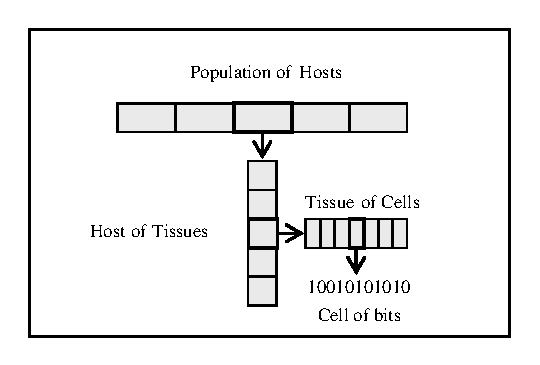
\includegraphics[scale=0.85]{Framework/framework-clonalselection-hierarchy-expansion}
	\caption{Depiction of an expanded realisation of a hierarchical clonal selection system with all three tiers.}
	\label{fig:framework:hcsf:expanded}
\end{figure}


% Component Interaction
%
\subsubsection{Component Interaction}
This section provides a complement to the analysis of cardinality bracketing by considering the bracketing of the interactions of the structures under adaptation across the investigated paradigms and algorithms. Interaction refers to direct competition or pattern recognition between structures (such as in the cellular paradigm), or the communication of information between structures (such as in the tissue and host paradigms). Bracketing of interaction refers to the specific constraints imposed on the interaction between structures at different scales within clonal selection algorithms. Table~\ref{tab:framework:hcsf:interaction} provides a summary of which components interact across the algorithms of the three paradigms. The general algorithms for each paradigm, specifically CCSA, DCCSA, TCSA, PHCSA, and GHCSA explicitly list interactions for all structures, whereas specialised algorithms list interactions only for relevant structures. 

\begin{table}[htp]
	\centering\small
		\begin{tabular}{llccccc}
		\toprule
		\textbf{Paradigm} & \textbf{Algorithm} & \textbf{c} & \textbf{C} & \textbf{T} & \textbf{H} & \textbf{P} \\ 
		\toprule
		\emph{Cellular} & DCCSA 			& yes & no & no & no & no \\ 										
									  & CCSA 				& yes & yes & no & no & no \\ 
									  & MCCSA 			& no & no &  &  &  \\
									  & $\ast$CCSA	& no & yes &  &  &  \\
		\midrule
		\emph{Tissue} & TCSA 				& yes & yes & yes & no & no \\ 
								  & MTCSA 			&  & yes & no &  &  \\ 
								  & $\ast$TCSA 	&  & yes & yes &  &  \\ 								  
		\midrule
		\emph{Host} & PHCSA 				& yes & yes & yes & yes & no \\ 
								& MP-HCSA 	 		&  & yes & no & no &  \\ 
								& $\ast$PHCSA 	&  & yes & no & yes &  \\ 							
								& GHCSA 				& yes & yes & yes & yes & yes \\ 
								& MG-HCSA  			&  & yes & no & no & no \\ 
								& $\ast$GHCSA 	&  & yes & no & no & yes \\ 								
		\bottomrule
		\end{tabular}
	\caption{Summary of the component interaction across the abstract and realised clonal selection algorithms, where $\ast$ represents a wild-card for descendant algorithms of a given base algorithm.}
	\label{tab:framework:hcsf:interaction}
\end{table}

% cardinality
Naturally, the suggested and adopted bracketing of interactions mirrors the bracketing of cardinality. Restricting cardinality was designed to directly restrict the effects of interaction, and the elaboration of the cardinality was designed to directly provide a context for investigation.
% need cells
An important point implicit in the bracketing of cardinality and explicit in the interactions is that cells and their interactions are required (almost) universally by all clonal selection algorithms, with the DCCSA as the single exception. This is because the structures under adaptation at higher levels of abstraction ultimately all subsume cells, specifically receptors on and excreted by cells. Beyond the verification of the primary objects of the adaptive systems formalism discussed in Section~\ref{sec:framework:hcsf:comparison}, this reinforces the fact that both the clonal selection theory and the inspired computational principles are defined in a cellular context. The implications of this fact reinforces the `perspectives on the clonal selection adaptive strategy' consideration of the three investigated paradigms in this work. 
% minimum algorithms
The interactions between structures was defined in Section~\ref{sec:framework:hcsf:comparison} as the operators providing the defining characteristic between strategies within each paradigm. This is highlighted in the naming convention adopted where the \emph{Minimum} of each algorithm class is defined with no interaction between the structures under adaptation, providing a baseline for comparison of the effects of such interactions.


%
% Summary
%
\subsection{Summary}
\label{sec:framework:hcsf:summary}
The integration and analysis of the three clonal selection paradigms with a compressed antigenic exposure paradigm in the HCSF provided a context for both (1) retrospectively explaining generalised design and methodology principles for clonal selection algorithms, and (2) promoting consideration of permutations of cardinality and interaction that although are predicted by the framework were not investigated in this work. This section reviews the explanatory and predictive power of the `system biased' Hierarchical Clonal Selection Framework, as follows:

\begin{enumerate}
	% Explanatory
	\item \emph{Explanatory Power}
	\begin{enumerate}
		\item \emph{Cellular Basis}: Irrespective of the specific perspective taken (level of abstraction), the clonal selection theory and computational principles is a bottom-up pattern recognition-based adaptive strategy involving cells (receptors or detectors) and antigen (complementary structures).		
		\item \emph{Bracketing}: The forward and backward bracketing of the cardinality in the context of a hierarchical complex adaptive system has been demonstrated to provide a powerful tool for investigating such a system.
		\item \emph{Naming Conventions}: A perspective invariant naming convention promotes the naming of the perspective for the structures under adaptation, and the design of a minimal strategy of bracketed interactions between such structures as a baseline for measure the effects of such interactions.		
	\end{enumerate}
	
	% Predictive
	\item \emph{Predictive Power}
	\begin{enumerate}
		\item \emph{Varied Bracketing}: An analysis of the specific bracketing considered in the investigation highlighted the bracketing that was not considered, as well as the removal of bracketing all together to consider a broader hierarchical clonal selection system, providing a rich basis for future investigation.
		\item \emph{Compound Effects}: The investigation and application of an unbracketed clonal hierarchical selection based system provides an opportunity for identifying and assessing the compound and expected non-linear aggregate effects of cross-component and cross-tier interactions. 
		\item \emph{Alternative Perspectives}: The consideration of the three paradigms in aggregation provided a context to consider (1) the potential splitting of the Cellular and Host paradigms into new and/or sub-paradigms, and (2) suggested at the potential for perspectives of clonal selection not yet considered.
	\end{enumerate}	
\end{enumerate}


%
% Antigenic Exposure Framework
%
\section{Antigenic Exposure Framework}
\label{sec:framework:haef}

%
% Paradigms
%
\subsection{Paradigms}
\label{sec:framework:haef:paradigms}
% artificial relationship
The antigenic exposure paradigm was defined as a complement to the clonal selection strategy, and elaborated in scale along with the adaptive systems across the three paradigms. Although the clonal selection abstractions had a basis in reviewed immunophysiology, the antigenic environments were contrived from the general properties of endogenous and exogenous antigen. The reason for this was that although an antigenic environment is required to stimulate a clonal selection system, it was not the focus of the investigation. 
% this section
This section integrates all of the scales of the antigenic exposure paradigm investigated in this work from across the three paradigms, specifically: antigen (and determinants), antigenic infections, and antigenic habitats. The integration of these concerns is referred to as the \emph{Hierarchical Antigenic Exposure Framework (HAEF)}.
% integration
As with the hierarchical clonal selection framework, the focus of this integrated framework is on the explanatory and predictive power provided via an analysis of the constraints imposed (referred to as bracketing) at each level in the hierarchy. Unlike the clonal selection framework, this section is not concerned with comparing and contrasting the tiers in the context of an adaptive systems formalism. The reason for this is that the antigenic environment is not an adaptive system, rather a required component of the clonal selection adaptive system.
% perspective
As such, the perspective on the antigenic environments is elaborated, compressing the concerns of clonal selection to provide an inverse perspective as to that considered in the integration of clonal selection (Figure~\ref{fig:framework:haef:interpretation:flat-expanded})

\begin{figure}[htp]
	\centering
	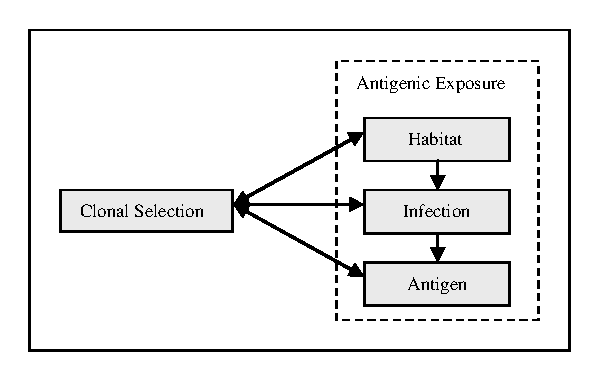
\includegraphics[scale=0.85]{Framework/framework-integration-flat-expanded}
	\caption{Depiction of the focus on environment and the compression of the systems in the Hierarchical Antigenic Exposure Framework (HAEF).}
	\label{fig:framework:haef:interpretation:flat-expanded}
\end{figure}

%
% Bracketing Analysis
%
\subsection{Bracketing Analysis}
\label{sec:framework:haef:bracketing}
Bracketing in the antigenic exposure paradigm involved constraints imposed on the cardinality of the \emph{triggers for adaptation} and the regimes that governed the piece-wise exposure of environmental information to a given system. This section considers the bracketing of configurations imposed on these two antigenic environment concerns.

%
% Component Cardinality
%
\subsubsection{Component Cardinality}
% bracketing
The bracketing of the cardinality of the information in the environment was configured to match the scale of the units of adaptation in the adaptive systems. Unlike clonal selection, the antigenic environment was not motivated in its interaction with the systems (for example adversarial, dynamic, and/or adaptive). The neutrality of the environment was intentional to focus attention on the emergent system behaviour under low-complexity environment concerns. 
% table
Table~\ref{tab:framework:haef:bracketing:cardinality} summarises the cardinality of the abstract antigenic environments and the realised colour space antigenic environments in terms of the previously defined: determinants ($D$), antigen ($A$), infections ($I$), habitats ($B$) and environments ($E$). 

\begin{table}[htp]
	\centering\small
		\begin{tabular}{llccccc}
		\toprule
		\textbf{Paradigm} & \textbf{Problem} & \textbf{D} & \textbf{A} & \textbf{I} & \textbf{B} & \textbf{E} \\ 
		\toprule
		\emph{Cellular} & AEP 	& N & N & 1 & 1 & 1 \\ 
									  & ACSP 	& 1 & N & 1 & 1 & 1 \\ 
									  & DCSP 	& N & N & 1 & 1 & 1 \\
		\midrule
		\emph{Tissue} & IAEP 		& N & N & N & 1 & 1 \\ 
									& ICSP 		& 1 & 1 & N & 1 & 1 \\ 
		\midrule
		\emph{Host} & HAEP 			& N & N & N & N & 1 \\ 
								& HCSP 			& 1 & 1 & 1 & N & 1 \\ 
		\bottomrule
		\end{tabular}	
	\caption{Summary of the component cardinality across the principle abstract and realised antigenic exposure problems.}
	\label{tab:framework:haef:bracketing:cardinality}
\end{table}

% levels
The table shows the potential of each abstract exposure problem and the strong bracketing of the colour space realisations for the structures under adaptation in the systems in each tier of the hierarchy. 
% equivalent levels
The ACSP, ICSP, and HCSP all exploited the same bracketing method, specifically the treating of each Colour Space Pattern (colour) as a trigger for adaptation at the respective tier. For example, a set of antigen (ACSP) is equivalent to a set of infections (ICSP) and a set of habitats (HCSP), in that they can all be reduced to a set of Colour Space Patterns.
% reason
This equivalence in problem was designed to minimise the complexity of the information to be acquired across the tiers to a level that was easy to interpret, whilst introducing complexity the way in which the information was exposed and expected through varied exposure regimes.
% alternative
This simplification of problem motivated the corresponding cross-cutting cellular-based clonal selection concerns in the systems by reducing all information to single antigen. One may consider the alternative of such a minimisation in a less constrained colour space realisations of the the exposure problems. For example, an infection of antigen may involve sets of antigen that are similar (intra-infection), although distinctly different between the sets (inter-infection). This could be realised through minor variations for intra-infection colour space patterns (similar colour), and major variations for inter-infection Colour Space Pattern centroids (inter-infection). This same example scales to the habitat level, with sets of sets of antigen, where intra-habitat infections may be more similar than inter-habitat infections. 
% what the simplification
These examples highlight what the bracketed cardinality provided, specifically exemplar patterns (set size of one with no variations) for each infection and habitat with promoted inter-trigger dissimilarity (minimum hamming distance).
% effect
This chosen level of cardinality bracketing had the effect of removing the degeneracy, (specifically the redundancy of the triggers of adaptation) requiring an immune response for each antigenic trigger in the antigenic environments. The alternatives provide an opportunity for re-introducing such degeneracy although at the cost of the specificity of a system in an environment (generalised response against variations for each antigenic determinant at the lowest level).

%
% Exposures
%
\subsubsection{Exposure Regimes}
% exposures
Antigenic exposure controlled the piece-wise revealment of information to the systems as well as the piece-wise spatial and temporal expectation of future exposure. In the context of forced response to a fixed information environment, the exposure regimes managed the complexity of the problems to be addressed by the systems. The complexity of exposure scaled with the increase in the level of abstraction starting with exposures, multiple exposures and multiple antigen in the definition of the exposure paradigm (Section~\ref{subsec:cells:paradigm:antigenicexposures}), and the raise in the level of abstraction of such exposures to include spatial concerns across multiple points of exposure in infection exposures (Section~\ref{subsec:tissues:paradigm:exposures}) and habitat exposures (Section~\ref{sec:hosts:paradigm:exposures}).
% this section
This section considers the bracketing of exposures with regard to (1) the spatial points of exposure, and (2) the temporal concerns of the expectation of exposure.

\begin{table}[htp]
	\centering\small
		\begin{tabular}{lllllll}
		\toprule
		\textbf{Paradigm} & \textbf{Problem} & \textbf{D} & \textbf{A} & \textbf{I} & \textbf{B} & \textbf{E} \\ 
		\toprule
		\emph{Cellular} & AEP & N & N & 1 & 1 & 1 \\ 
		 & ACSP 							& 1 & N & 1 & 1 & 1 \\ 
		 & DCSP 							& N & N & 1 & 1 & 1 \\ 
		\midrule
		\emph{Tissue} & IAEP 	& N & N & 1-N & 1 & 1 \\ 
		 & ICSP 							& 1 & N & 1-N & 1 & 1 \\ 
		\midrule
		\emph{Host} & HAEP 		& N & N & 1 & 1-N & 1 \\ 
		 & HCSP 							& 1 & N & 1 & 1-N & 1 \\ 
		\bottomrule
		\end{tabular}
	\caption{Summary of the bracketing of spatial exposure across the abstract and realised antigenic exposure problems.}
	\label{tab:framework:haef:bracketing:exposures:spatial}
\end{table}

% spatial exposure
Table~\ref{tab:framework:haef:bracketing:exposures:spatial} considers the bracketing of the spatial concerns of an exposure, in particular the triggers for adaptation in terms of the scope of the points of exposure in a system (1 or many). A point of exposure in a system is unit of adaptation, therefore given the chosen cardinality bracketing in both systems and environments, there is always a many-to-many relationship between the \emph{units} and \emph{triggers} of adaptation at the focused level of detail in the hierarchy.
% antigen
At the antigen level, the scope of the system (all points of exposure) is always exposed. This has the effect of requiring a mechanism to constrain a polyclonal activation (shown to be strong selection in Section~\ref{sec:cells:ccsa:dcsa}). The reason for this design decision was the relative small scale of a single repertoire of cells in the context of multiple of such repertoires (tissues) and multiple such hosts of tissues. The same strong selection was required at the determinant level, and given the antigen focus at all levels, this had the effect of requiring explicit aggregation of response toward holistic solution to address the resultant polyclonal response.
% tissues and hosts
This unbounded antigen-cell exposure and explicit strong selection and aggregation is bracketed in the tissue and host levels in the introduction of discrete Antigenic Exposure Regimes (AER) providing deterministic and probabilistic patterns of interaction between the units and triggers of adaptation (referred to as $1-N$ in the table). This had the effect of requiring the systems under such regimes to manage the spatial organisation (localisation and dissemination) of acquired information to best address the patterned interaction.
% spatial cells
One may consider the alternatives of such bracketing of spatial exposure, for example the spatial selection of cells in a repertoire considered in spatial up-front selection in Section~\ref{sec:cells:spatial}. The symmetrical exposure regime at the tissue (STER) and at the host (SHER) levels provide a counter example of the effects of simplifying exposure complexity to that of system-wide with respect to the points of exposure of a system.

\begin{table}[htp]
	\centering\small
		\begin{tabular}{lllllll}
		\toprule
		\textbf{Paradigm} & \textbf{Problem} & \textbf{D} & \textbf{A} & \textbf{I} & \textbf{B} & \textbf{E} \\ 
		\toprule
		\emph{Cellular} & AEP 	& N & N & 1 & 1 & 1 \\ 
		 & ACSP 						  	& N & N & 1 & 1 & 1 \\ 
		 & DCSP 								& N & N & 1 & 1 & 1 \\ 
		\midrule
		\emph{Tissue} & IAEP 		& N & N & N & 1 & 1 \\ 
		 & ICSP 								& N & N & N & 1 & 1 \\ 
		\midrule
		\emph{Host} & HAEP 			& N & N & N & N & 1 \\ 
		 & HCSP 								& N & N & N & N & 1 \\ 
		\bottomrule
		\end{tabular}
	\caption{Summary of the bracketing of temporal exposure across the principle abstract and realised antigenic exposure problems.}
	\label{tab:framework:haef:bracketing:exposures:temporal}
\end{table}

% temporal exposure
Spatial exposures without a time component are a compression of the patterns of exposure over the scope of the units of adaptation. Therefore, temporal exposures can be considered an opposite case of the compression of spatial location and a focus on the systems expectation of information on a timeline. Table~\ref{tab:framework:haef:bracketing:exposures:temporal} summarises the temporal expectations of the abstract and realised exposure problems with regard to the triggers for adaptation. The table clearly shows that the temporal expectations of exposure extended backward through the hierarchy from the focus of each tier. This simple but important perspective on the antigenic exposure paradigm highlights the motivating complexity for the corresponding Hierarchical Clonal Selection Framework, specifically the compounded increase in temporal expectation of information. This table also highlights the need for bracketing the information cardinality of antigenic environments across the hierarchy to bound the complexity of the effects of the compounded temporal expectations. 


%
% Summary
%
\subsection{Summary}
\label{sec:framework:haef:summary}
The integration and analysis of the antigenic exposure paradigm across the three levels of abstraction in the context of a compressed clonal selection system provided a context for both (1) retrospectively explaining generalised design and methodology principles for the of the problems that motivated the investigation of clonal selection algorithms, and (2) promoted the consideration of permutations and relaxation of cardinality, spatial, and temporal concerns of antigenic exposure. This section reviews the explanatory and predictive power of the Hierarchical Antigenic Exposure Framework, as follows:

\begin{enumerate}
	% Explanatory
	\item \emph{Explanatory Power}
	\begin{enumerate}
		\item \emph{Forced Response}: The strong bracketing of the cardinality of antigen across the hierarchy resulted in a forced response expectation from systems with regard to the trigger for adaptation. Such forced response may be relaxed by loosening the bracketed cardinality constraints at a given tier in the hierarchy, in particular for the infection and habitat levels.
		\item \emph{Compounded Expectation}: The focus of the investigation using the antigenic exposure paradigm was on compounded expectation with varied spatial scope of exposure at the tier of interest, and strong bracketing of the spatial scope at tiers above and below the tier of interest.
	\end{enumerate}

	% Predictive
	\item \emph{Predictive Power}
	\begin{enumerate}
		\item \emph{Cardinality Complexity}: An alternative to the design of clonal selection systems in response to exposure complexity, is that the design of such systems can be motivated by variations in the cardinality complexity instead and/or combinations of cardinality and exposure complexity. Specific examples of cardinality complexity include sets of antigen in each antigenic infection, and sets of infections in each antigenic habitat.
		\item \emph{Compounded Spatial Scope}: The spatial scope of exposure was constrained at tiers of the hierarchy above and below a focused level, the relaxation of this bracketed spatial exposure will provide an additional axis of problem complexity to explore in addition to compounded expectation.		
	\end{enumerate}	
\end{enumerate}


%
% Integrated Hierarchical Framework
%
\section{Integrated Hierarchical Framework}
\label{sec:framework:ihcsf}

%
% Frameworks 
%
\subsection{Frameworks}
\label{sec:framework:ihcsf:frameworks}
% this section
Given an assessment of integrated hierarchical clonal selection and antigenic exposure frameworks, this section considers the aggregation of the two frameworks towards a unified abstraction and framework for clonal selection in the context of an antigenic environment. This is a natural integration as the abstract and realised problems and algorithms in both sides of the integration were designed as a natural fit for each other.
% frameworks
This integration is referred to as the \emph{Integrated Hierarchical Clonal Selection Framework (IHCSA)} to differentiate it from the concerns of either independent framework, and to highlight the strong bottom-up clonal selection focus. 
% both sides perspective
As such, the focus of the framework is the hierarchical integration of the elaborated concerns of both the system and the environment, depicted in Figure~\ref{fig:framework:ihcsf:interpretation:expanded-expanded}

\begin{figure}[htp]
	\centering
	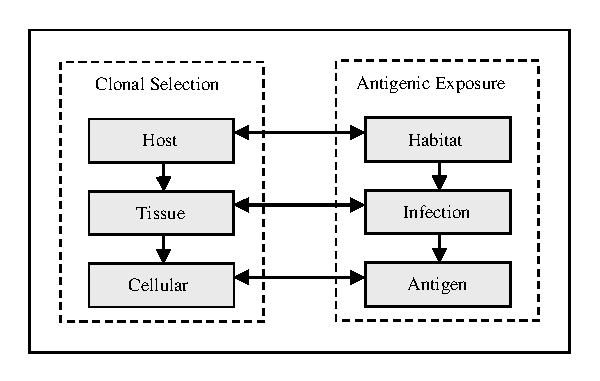
\includegraphics[scale=0.85]{Framework/framework-integration-expanded-expanded}
	\caption{Depiction of the focus on system and environment in the Integrated Hierarchical Clonal Selection Framework (IHCSF).}
	\label{fig:framework:ihcsf:interpretation:expanded-expanded}
\end{figure}


%
% Bracketing Analysis
%
\subsection{Bracketing Analysis}
\label{sec:framework:ihcsf:bracketing}
% section
This section focuses on the bracketing of concerns that have an effect both on the system and environment hierarchies. Specifically, this section is concerned with the matching or integrated cardinality across the hierarchy, and the effect of variations of this matching. Also considered in this section is the extension of the framework through the integration of additional tiers to the existing framework.

%
% Integrated Cardinality
%
\subsubsection{Integrated Cardinality}
\label{subsec:framework:ihcsf:bracketing:cardinality}
% section
The focus of this subsection is the bracketing of the cardinality of both the system and environment hierarchies as they pertain to the interaction between the hierarchies. Specifically, the interaction of the triggers for adaptation with the structures under adaptation at both the scope of their intended focus (for example cells and antigen in the cellular level), and scopes above and below that focus.

\begin{table}[htp]
	\centering\small
		\begin{tabular}{lccccc}
		\toprule
		 & \emph{c} & \emph{C} & \emph{T} & \emph{H} & \emph{P} \\ 
		\toprule
		\emph{D} & 1 & N & N & N & N \\ 
		\emph{A} &  & 1 & N & N & N \\ 
		\emph{I} &  &  & 1 & N & N \\ 
		\emph{B} &  &  &  & 1 & N \\ 
		\emph{E} &  &  &  &  & 1 \\ 
		\bottomrule
		\end{tabular}
	\caption{Summary of the suitability match between clonal selection and antigenic exposure components}
	\label{tab:framework:ihcsa:suitability}
\end{table}	

% ideal case
Table~\ref{tab:framework:ihcsa:suitability} summarises the intended or so-called ideal integrated cardinality cases for the environmental triggers and system units of adaptation. The table clearly shows the response suitability in terms of the one-to-one relationships (upper limit) and the general capability in terms of the one-to-many relationship of system structures to environmental triggers. It should be pointed out that the upper limit (one-to-one) of the suitability between the frameworks was not investigated throughout this work as an initial assessment may suggest. For example the cellular paradigm considered a `\emph{tissue of cells}' against an `\emph{infection of antigen}' rather than a cell against an antigen or the mismatch case of a `tissue of cells' against a single antigen. 
% investigated
Table~\ref{tab:framework:ihcsf:cardinality} elaborates on the ideal cases, and summarises the components of each hierarchy and indicates the scope of concerns of each paradigm, and the cases that were embodied in algorithms that were investigated (bold). Paradigms are marked with the first letter of the structures under adaptation, with the division of Cellular into Degenerate (D) and Cellular (C), and Host into Host (H) and Generational (G). Perspectives or tiers are defined by the interaction of the designated triggers and structures for each paradigm, for example cells (C) and antigen (A) in the cellular paradigm. The italicised cases demonstrate those cases that could be addressed from tiers above and below a given tier.

\begin{table}[htp]
	\centering\small
		\begin{tabular}{llcccccccccc}
		\toprule
		 &  & \multicolumn{2}{c}{\textbf{c}} & \multicolumn{2}{c}{\textbf{C}} & \multicolumn{2}{c}{\textbf{T}} & \multicolumn{2}{c}{\textbf{H}} & \multicolumn{2}{c}{\textbf{P}} \\ 
		\toprule
		 &  		 &    $1$ & $N$ & $1$ & $N$ & $1$ & $N$ & $1$ & $N$ & $1$ & $N$ \\ 
		\midrule
		\textbf{D} & $1$ & D & D &   &   &   &   &   &   &   &  \\ 
		 				 & $N$ &   & \textbf{D} & \emph{C} & \emph{C} &   &   &   &   &   &  \\ 
		\midrule
		\textbf{A} & $1$ & 	 & \emph{D} & C & C &  &   &   &   &   &   \\ 
		 				 & $N$ & 	 &   &   & \textbf{C} & \emph{T} & \emph{T}  &   &   &   &   \\ 
		\midrule
		\textbf{I} & $1$ &   &   &   & \emph{C} & T & T &   &   &   &   \\ 
		 				 & $N$ &   &   &   &   &   & \textbf{T} & \emph{H} & \emph{H}  &   &   \\ 
		\midrule
		\textbf{B} & $1$ &   &   &   &   &   & \emph{T} & H & H &   &   \\ 
		 				 & $N$ &   &   &   &   &   &   &   & \textbf{H} & \emph{G} & \emph{G}  \\ 
		\midrule
		\textbf{E} & $1$ &   &   &   &   &   &   &   & \emph{H} & G & \textbf{G} \\ 
		 				 & $N$ &   &   &   &   &   &   &   &   &   & G \\ 
		\bottomrule
		\end{tabular}
	\caption{Summary of the component cardinality for both the clonal selection and antigenic exposure models.}
	\label{tab:framework:ihcsf:cardinality}
\end{table}

% minimum maximum
An important point highlighted by this table are the overlapping concerns between the paradigms. For example $N$ cells may be regarded as a single tissue (minimal cardinality tissue model), both of which can address $N$ antigen or 1 infection (minimum cardinality infection model). The designed subsumption inherent in both independent and the integrated frameworks promote this \emph{maximum-minimum principle} at the transitions between tiers in the hierarchy. This principle allows similar concerns to be investigated from two different perspectives. For example in the cellular-tissue case, one can investigate the the systems composition and capability of a repertoire in response to a set of $N$ antigen with explicit aggregation of the best matching cells for each antigen from the cellular perspective, or the response capabilities of a tissue against a single antigen from the tissue perspective. Both examples provide a different context (different level of abstraction with regard to the acquired immune system) that may provide varied strategies for considering the same problem. The table clearly shows such cases were investigated using the maximum of the previous tier rather than the minimum of the given tier. 
% what was investigated
The highlighting of investigated cases clearly shows the scope of future work with regard to integrated cardinality cases. An interesting point is that the generational case did not follow the trend and investigate multiple environments with multiple populations. Rather, the EI-HCSA adapted multiple populations against a single antigenic environment (set of habitats). 
% not investigated in scope
The table also provides a clear indication of those cases delineated to specific scopes of interest that were not investigated, and those cases that could not be investigated. For example, the maximum trigger for a given tier ($N$) with the minimum structures of adaptation (1) is an infeasible combination defining the upper limit on cardinality complexity for each system.

% classical integrated cardinality picture
\begin{figure}[ht]
	\centering
	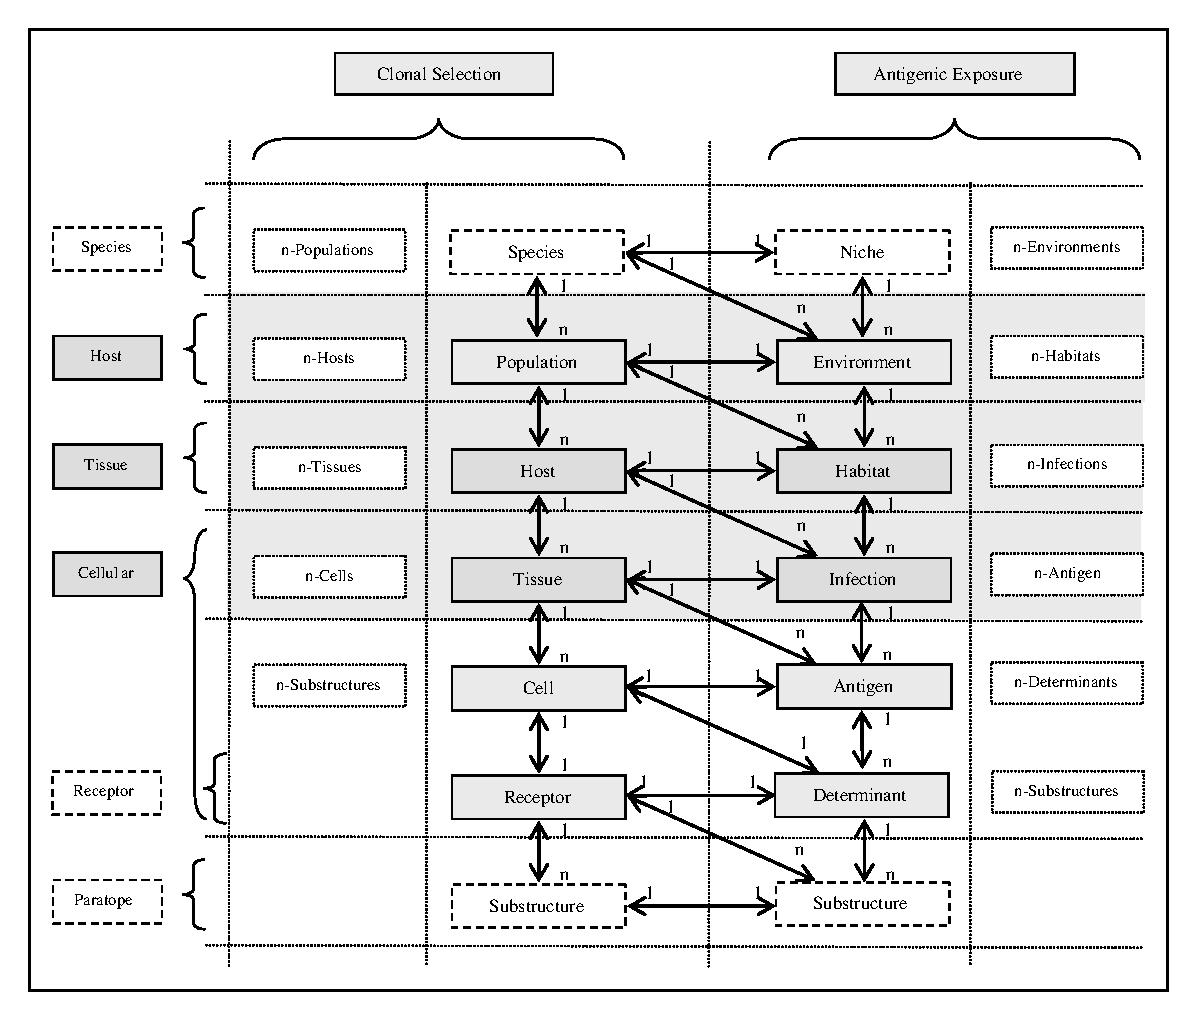
\includegraphics[scale=0.75]{framework/framework-integrated-cardinality}
	\caption{Depiction of the integrated hierarchical clonal selection and hierarchical antigenic exposure frameworks, showing subsumed relationships and component cardinalities across the investigated paradigms.}
	\label{fig:framework:ihcsf:cardinality}
\end{figure}

% picture
Figure~\ref{fig:framework:ihcsf:cardinality} depicts the integrated cardinality bracketing in a hierarchical way to enforce the subsumed responsibility across the tiers, providing a standard representation of the frameworks and basis for extrapolating from the integrated relationships. The figure is information dense capturing intra- and inter-tier relationships for both the system and environment frameworks, and clearly highlighting the important maximum-minimum principle at tier-boundaries (diagonal lines). 
% receptors 
An interesting observation is that of the relationship between the cells and antigen, showing that a cell and a receptor do not differ in terms of their information content, and that a cells receptor is specialised for a given determinant on an antigen (base principles of the clonal selection theory). This is important given the compression of this relationship (bracketing) of one-antigen-to-one-determinant (and thus one receptor or cell) throughout the majority of the investigations. Only the DCCSA considered the relaxation of this bracketing, allowing cells (receptors) to be selected for by the determinants of an antigen. This specialisation was classified as apart of the cellular paradigm, although if such specialisations are elaborated and investigated (specifically the one-to-many relationship between an antigen and receptors as in the DCCSA in Section~\ref{sec:cells:ccsa:dcsa}), one may refer to this as the \emph{Receptor Clonal Selection Paradigm (RCSP)} to clearly distinguish it from the cellular paradigm.
% additional tiers
The figure also suggests at tiers above and below the the host and tissue tiers respectively, outside of the scope of what was investigated. These extrapolated additional tiers are considered in the next section.


%
% Additional Tiers
%
\subsubsection{Additional Tiers}
\label{subsec:framework:ihcsf:bracketing:additionaltiers}
A point stressed in the integration of the three investigated clonal selection paradigms in this Chapter has been that each represents a single perspective on the application of clonal selection as an adaptive strategy. Explicitly selected in the standard form depiction of the integration in Figure~\ref{fig:framework:ihcsf:cardinality} was the capability for additional vertical tiers above and below the host and cellular tiers respectively, as well as the potential for integration of additional perspectives of a given tier. This section extrapolates examples of such additional perspectives on clonal selection and integrates them into the hierarchical framework of such perspectives.

%
% Population Clonal Selection
%
\paragraph{Population Clonal Selection}
A perspective beyond that of a population of hosts and an environment of habitats may be that of a \emph{species} and an ecological \emph{niche}, where a a set of populations interacts with a set of environments called the \emph{Population Clonal Selection Paradigm (PCSP)}. Like the generational variation of the host paradigm, the population paradigm involves maintenance of populations as the structures of adaptation, although the separation between the populations is spatial rather than temporal. As a tier beyond the host level, it subsumes the concerns of the host level including the generational turn-over, introducing inter-population interaction concerns such as those from population genetics (such as migration), and epidemiology (such as the spread of disease).

%
% Paratope Clonal Selection
%
\paragraph{Paratope Clonal Selection}
Given that the clonal selection theory describes the observations of immune cells, a level below the cellular level may not be a reasonable proposition. One may consider the development of a single receptor of sub-structures for a single antigenic determinant of sub-structures as the maximum in complexity of this preceding tier. The scale of the process is that of the tertiary confirmation of the immunoglobulin proteins and related immunochemical forces of their interaction with complementary structures of the determinants on macro-molecules and proteins, governed by the sequence amino acids that make up both molecules. This tier is referred to as the \emph{Paratope Clonal Selection Paradigm (ACSP)}\footnote{Paratope was chosen as the term for a sub-structure of a receptor molecule for lack of a better term.} and may be concerned with the specific chemical basis for immunoglobulin synthesis in cells, the valance of immunoglobulin molecules, and the physical forces that govern the molecular interactions and resultant affinity and avidity for determinants.

%
% Summary
%
\subsection{Summary}
\label{sec:framework:ihcsf:summary}
This final hierarchical integration represents the pinnacle of the abstractions presented. The integration and analysis of the integration framework provided a context for both (1) retrospectively explaining generalised design and methodology principles that motivated the investigation of clonal selection algorithms, and (2) promoted the consideration of unrealised permutations and relaxation of cardinality and additional tiers of the framework. This section reviews the explanatory and predictive power of the Hierarchical Integrated Clonal Selection Framework, as follows:

\begin{enumerate}
	% Explanatory
	\item \emph{Explanatory Power}
	\begin{enumerate}
		\item \emph{Framework as a Map}: The integrated framework facilitates the \emph{explicit} specification of immunological and antigenic concerns in terms of their scope of influence relative to each other. 
		\item \emph{Maximum-Minimum}: Tier transitions are defined by the maximum cardinality complexity of one tier that is reduced to the minimum cardinality complexity of the next tier. Such boundaries allow the same information content (problem) to be addressed from the perspectives of the tiers above and below the boundary, revealing insights and alternative solution strategies.		
		\item \emph{Simplest Case}: The investigations considered the average case of each paradigm, specifically the many-to-many relationship between triggers for adaptation and units of selection and adaptation.
	\end{enumerate}
	
	% Predictive
	\item \emph{Predictive Power}
	\begin{enumerate}
		\item \emph{Varied Interpretation}: The backward competence of a paradigm with its subsumed levels suggests at non-contigious interpreted cases of cardinality and interaction along both the system and environmental axis. The realisation of such models facilitate the use of tier-specific mechanisms (algorithms) on backwardly-compatible (subsumed) problem domains. 
		\item \emph{Additional Tiers}: The integration of the frameworks facilitated the elaboration of the cellular and host tiers to include concerns beyond the scope of these two limits of the framework.
		\item \emph{Additional Mapping}: The extensibility of the framework suggests at the potential for mapping all manner of immunological and antigenic concerns into the appropriate scope of the framework and defining relationships in terms of cardinality and interaction of structures and triggers. For example, the Negative Selection, Danger Theory, and Immune Network Artificial Immune System paradigms.
	\end{enumerate}		
\end{enumerate}


%
% Hierarchical Methodology
%
\section{Methodology and Hierarchical Framework}
\label{sec:framework:ihcsf:applicability}
% section
The integrated Hierarchical Clonal Selection Framework was not conceived independently of the tiers of the framework, nor were the tiers conceived independently of each other, rather they were systematically co-developed. This section considers (1) an overview of the methodology used to develop and investigate the clonal selection framework, (2) the application of the framework as a template for investigation in the broader field of Artificial Immune Systems, and (3) the framework as a template for investigation in the separate but related Computational Intelligence sub-fields.

%
% Partition-Reduction Methodology
%
\subsection{Partition-Reduction Methodology}
\label{subsec:framework:ihcsf:applicability:methodology}

%
% Methodology Overview
%
\subsubsection{Methodology Overview}
% elucidated
In considering the applicability of the chosen hierarchy for clonal selection and the methodology for applying such a methodology, it is critical that the motivation and adopted methodology be clearly elucidated.
% general approach used
The general systems theoretic approach used involved three important considerations (1) the distillation of the core computational principles and strategy from the clonal selection theory,  (2) the division of the clonal selection concerns into that of \emph{system} and \emph{environment}, and (3) the reduction of the holistic acquired immune system to that of the cellular concerns of the clonal selection theory. These steps are summarised as follows:

% this may be phrased as a general methodology as follows:
\begin{enumerate}
	\item \emph{Metaphor}: Identify the relevant observations, theory, and abstractions of the selected metaphor.
	\item \emph{Strategy}: Distil the metaphor to the core computational principles and information processing strategy.
	\item \emph{Partition}: Divide the concerns from the principles and strategy into a framework of \emph{systems} and \emph{environments}.
	\item \emph{Reduction}: Relate the components and their interactions at the lowest and highest levels (within scope of the metaphor).	
\end{enumerate}

% distillation
The distillation of clonal selection theory resulted in an adaptive strategy concerned with information acquisition, the concerns of which were partitioned into the \emph{immune system} and the \emph{antigenic environment}. 
% reduction
The reduction from immune system to the cellular concerns of the theory focused on the three different and inter-related \emph{functional organisations} of cells under clonal selection: the simplest case of antigens and cells in a small group (\emph{cellular}), many groups of cells using structural concerns to influence antigenic interactions (\emph{tissue}), and groups of immune systems influencing the transmission of disease and evolving (\emph{host}). The selection of the levels in the reduction was also generally motivated based on the \emph{units of selection} consideration from selectionist theory, providing a cellular basis in the reduction given that the lymphocyte is the unit of selection and adaptation in the clonal selection theory.
% intra-tier reduction
Importantly, the general functional reduction was taken a step further by considering the cardinality of the units of selection and their interaction within each tier, and focusing on the limits of each.

%
% Relation to Methodologies
%
\subsubsection{Relation to Methodologies}
The adopted methodology is comprised of concerns of the three reviewed approaches for investigating biologically inspired computation, immune information processing, and adaptive systems in Section~\ref{sec:background:methodology}. This section briefly highlights the selected aspects of the motivating methodologies and how they contributed to the integrated adopted methodology.

% conceptual framework
The general approach was a realisation of the five-step conceptual framework from biologicall-inspired algorithms (\ref{subsec:methodology:conceptual}). Specifically (1) the selection of the immune system as the motivating metaphor, (2) the review of immunochemistry and immunophysiology (probes) as a basis for information processing principles, (3) the investigation of models as abstraction of the information processing properties from models, (4) the application and verification of the computational models (considered next in Chapter \ref{chap:iidle}), and (5) resulting computational tools. The adopted methodology drew heavily from this approach, in particular with regard to the general process for realising viable computational tools, and with regard to the strong focus on the transition from probes (\emph{metaphor}) to information processing models that were investigated (results of the reductions).
% immune information processing
The immune information processing approach (Section~\ref{subsec:iip}) provided a specific context to motivate the conceptual framework, in particular to focus on the information processing concerns of immunology.
Goldberg's so-called \emph{small models} methodology for adaptive systems (Section~\ref{subsec:smallmodels}) provided a strong influence in the adopted methodology, specifically focusing the modelling effort on the decomposition of general information processing to separate sub-problems (\emph{reduction}) and the ultimate re-integration (the IHCSF). Along with the reductionist consideration, Goldberg's methodology promoted a strong focus on the bracketing of high-order phenomena which was realised in particular with regard to the cardinality and interactions between structures.
% deviation
It is important to clarify that the \emph{small models} methodology anticipates system modelling is achieved through the use of mathematical methods. The approach taken in this work involved the use of algorithmic computational modelling and simulation. An additional alternative modelling approach that could have been used is diagrammatic object and state modelling, such as the Unified Modelling Language (UML).


%
% Alternative Interpretations
%
\subsubsection{Alternative Interpretations}
% consider alternatives
The specific reduction was an clonal selection-specific interpretation of the immune system based on the functional aggregation of cells at three intuitive levels of detail. This suggests that alternative cellular-based reductions may be considered, as well as reductions not based on the units of selection and adaptation in the clonal selection theory. 
% whole other ways
An additional consideration for a reduction may include an antibody protein focus perhaps including the concerns of other macromolecules that influence the behaviour of the immune system such as cytokines and cellular receptors for such self-molecules. This would provide a focus on the interaction of components for signalling rather than adaptation. Alternatively, one may focus on the division of the immune system into adaptive and innate, and focus on the structures and functions within each `sub-system' promoting a stronger consideration of the concerns of the innate immune system and its interrelated processes with the acquired immune system.
% other considerations for cell based
The viability of a given reduction may be assessed based on the insights it provides regarding the computational principles under consideration. As such, an alternative already considered is the `\emph{immune system} $\leftrightarrow$ \emph{cellular}' reduction common across paradigms in AIS, suggesting that the contributions of the IHCSF may be the host and tissue considerations and the levels of comparison they provide.

%
% Hierarchical Artificial Immune Systems
%
\subsection{Hierarchical Artificial Immune Systems}
\label{subsec:framework:ihcsf:applicability:ais}
The field of Artificial Immune Systems is concerned with the investigation of computational tools inspired by the structure and function of the immune system (see Section~\ref{sec:ais}). Given the pervasiveness of molecular and cellular concerns in immunology and the follow-on effects of this focus into Artificial Immune Systems, one may consider the application of the proposed Integrated Hierarchical Clonal Selection Framework as a general tool in AIS. Specifically, the hierarchical perspective may be used as a framework to focus effort for the integration existing seeming disparate computational methods inspired by immunology, and potentially highlighting new opportunities for investigating AIS.

%
% Negative Selection
%
\subsubsection{Negative Selection}
% negative selection
The negative selection paradigm exploits the clonal selection process for adaptation-based information acquisition although focus on the specific concerns of using pattern recognition to discriminate self from nonself and the preparation of such pattern detectors (see Section~\ref{subsec:background:negativeselection}).
% negative selection as strategy
% too provocative?
The first important consideration is that of negative selection as adaptive strategy (modelling in the complement space with centralised preparation and with decentralised opportunistic specialisation using clonal selection). The strategy focus of the paradigm highlights the constraints under which the strategy must operate (satisfice) within the immune system at varied levels of abstraction. Such consideration may provide insight to advance the paradigm beyond the current highly-constrained cellular perspective, and the limitations of such approach in practical application \cite{Stibor2006}. 

\begin{table}[htp]
	\centering\small
		\begin{tabularx}{\textwidth}{lX}
		\toprule
		\textbf{Scope} & \textbf{Negative Selection} \\ 
		\toprule
		\emph{Cellular} & Centralised detector generation and application. \\ 
		\midrule
		\emph{Tissue} & Centralised/Decentralised detector generation and decentralised application.\\ 
		\midrule
		\emph{Host} & Controlled antigenic exposure, biased restarts of environmental perspective, and adaptation of generation and application structures and processes. \\ 
		\bottomrule
		\end{tabularx}
	\caption{Summary of the Negative Selection AIS paradigm mapped onto the three tiers of the IHCSF.}
	\label{tab:framework:ais:negativeselection}
\end{table}

% clonal selection core
Table~\ref{tab:framework:ais:negativeselection} provides a summary of the mapping of the negative selection paradigm onto the IHCSF. Given the close ties with clonal selection, the negative selection paradigm has generally the same concerns. Specifically, effective adaptation in the cellular tier, and effective localisation and dissemination in the tissue and host tiers. 
% antigenic
Also consistent with the clonal selection paradigm is the antigenic environment, where the information in the environment encapsulates the scope of patterns that must be differentiated from self patterns. 
% self corpus
The important differences between the paradigms is the strong focus on cellular preparation required in negative selection that may be achieved locally or globally. 
%  cells
For example, the corpus of self-patterns may be centrally managed at the cellular scope providing a focus on effective non-self pattern generation, and the general application of such detectors.
% tissues
At the tissue scope, the preparation of the detectors may be centralised in a \emph{thymus model} where a specific centrally connected tissue is designated the role of managing the self-pattern corpus and detector generation, with system-wide decentralised application and localised refinement of the recirculated detectors. Alternatively the management of the corpus may decentralised and distributed throughout the tissues of the system for localised (specialised) preparation and dissemination, likely a more scalable configuration, particularly if the self corpus is accumulated in an opportunistic manner. These concerns were considered by Hofmeyr in his dissertation (see Section~\ref{subsubsec:distrb:review:security}) and provide a important research agenda for negative selection \emph{at the tissue scope of the integrated hierarchy}. 
% host
The host has similar concerns as that of the tissue, although with the important shift in focus from a strongly integrated series of perspectives to strongly independent holistic perspectives with weak integration. Pattern generation is centralised within each perspective although some control is provided over the exposure to information, the restarting of perspectives with biasing, and the long-term adaptation of the structure and processes of detector preparation and application.

%
% Immune Network
%
\subsubsection{Immune Network}
% immune network
The immune network paradigm is concerned with intra-receptor interactions with and without the presence of antigen and was proposed to be a specialised case of clonal selection at the cellular level (Section~\ref{sec:cells:network}). This paradigm was investigated (1) briefly, and (2) only at the cellular level, suggesting an opportunity for further elaboration and integration with the scope of artificial immune network approaches.
% strategy
The information processing strategy distilled form the theory was that of repertoire maintenance using intra-cellular interactions. Such interactions form networks of cellular relationships which may be considered intra-repertoire higher order structures, that may be exploited for storing more complex information.

\begin{table}[htp]
	\centering\small
		\begin{tabularx}{\textwidth}{lX}
		\toprule
		\textbf{Scope} & \textbf{Immune Network} \\ 
		\toprule
		\emph{Cellular} & Formation and maintenance of intra-repertoire relationships. \\ 
		\midrule
		\emph{Tissue} & Interaction and integration of inter-tissue cell-based relationships. \\ 
		\midrule
		\emph{Host} & Generational refinement of structures as well as the processes and structures used to form and maintain such structures. \\ 
		\bottomrule
		\end{tabularx}
	\caption{Summary of the Immune Network AIS paradigm mapped onto the three tiers of the IHCSF.}
	\label{tab:framework:ais:immunenetwork}
\end{table}

% breakdown
Table~\ref{tab:framework:ais:immunenetwork} provides a summary of the mapping of the immune network strategy to the three tiers of the IHCSF. 
% antigen and relationships
The antigenic environment involves the scope of the standard clonal selection antigenic environment at each tier in the framework, in addition to the scope of intra-repertoire interactions that may result. As these relationships are scaled-up from the cellular level, they may be considered to occur between tissues, and between hosts, with the latter providing a truly abstract proposition for the theory. 
% tissue
From the tissue perspective, the localisation and dissemination of acquired information extends from information about antigenic infections, to information about the relationships within each tissue. The dissemination of cells involved in inter-cell relationships provides an opportunity for the interaction and ultimate integration of localised relationships between tissues, providing new contexts for response, and likely initially disrupting the maintenance of localised relationships. 
% host
The host perspective, in particular the generational specialisation provides a context for considering the biasing (so-called `seeding') of cellular relationships, and ongoing refinement of these relationships over extended time periods across multiple host-lineage in a population using the maternal immunity approach. The generational specialisation also provides an opportunity for adapting the processes and structures used in the formation and maintenance of relationships, allowing potentially for the development of new relationship types (structures).

%
% Other
%
\subsubsection{Other}
The generality of the reduction of functional immunology from the scope of a holistic immune system to the theory-laden cellular level may provide a powerful abstraction for many unrealised and/or budding Artificial Immune Systems. Examples may include, danger theory, innate immunity, cytokine molecules, and the large number of cell types and their interactions. The so-called power of the abstraction comes from (1) the context it provides for framing the information processing qualities of an immunological structure or process, (2) the strong focus on identifying and bracketing of complexity in resultant models promoting clear schedule for experimentation and elaboration, and finally, (3) a context for the integration of findings into a coherent model of the motivating paradigm. 

%
% Hierarchical Framework Methodology
%
\subsection{Hierarchical Framework Methodology}
\label{subsec:framework:ihcsf:applicability:other}
% section
This section considers the exploitation of the proposed methodology in different but related biologically-inspired Computational Intelligence sub-fields. In considering this question, a brief assessment of two general fields are considered, specifically (1) \emph{Evolutionary Computation} and (2) \emph{Connectionist Intelligence}. The fields are considered in the context of their \emph{metaphor}, \emph{strategy}, \emph{partitioning} into system and environment, and \emph{reduction}. 
% expectation
Given the enormity of the research into the selected Computational Intelligence sub-fields the hierarchical phrasing of the three adaptive strategies is not likely to reveal any insights into the respective paradigms, rather the expectation is that the reductionist methodology may provide a framework for better integrating findings from existing approaches. 


%
% Evolutionary Computation
%
\subsubsection{Evolutionary Computation}
% metaphor
The metaphor for the well studied evolutionary computation field is neo-Darwinian evolution, taking into account the genetic concerns of micro- and macroevolution.
% strategy
The distilled computational principles include selection and descent with modification typically via the recombination and mutation of structures. The computational strategy may be summarised as adaptation toward relative improvement under the constraints of an environment (see Section \ref{subsec:cs:related:ec}). 
% division
The summation of the adaptive strategy highlighted the intuitive separation of the population of structures under adaptation, and a environment responsible for defining the scope of `fitness', typically apportioned directly in terms of quantitative scalar values that are interpreted by the adaptive strategy as the proportionate allocation of available resources.
% reduction
Table~\ref{tab:framework:other:ec} provides a summary of an interpreted reduction of evolution from the species level to the DNA level, constraining both the general adaptive strategy and fitness-assigning environment.
% why the specific division
The reduction is based on the units of selection and adaptation using the same general approach as was adopted in the reduction of clonal selection. The chosen units of selection include genomes, populations, and species, which forms an Integrated Hierarchical Evolutionary Framework. 

\begin{table}[htp]
	\centering\small
		\begin{tabularx}{\textwidth}{llX}
		\toprule
		\textbf{Tier} & \textbf{Environment} & \textbf{System} \\ 
		\toprule
		\emph{Genome} & Habitat of Localities. & \emph{Population of Genomes}, adapting in context of the scope of information being adapted and its mapping to an assessable form. \\ 
		\midrule
		\emph{Population} & Niche of Habitats. & \emph{Species of Populations}, localising and disseminating adapted genomes.\\ 
		\midrule
		\emph{Species} & Ecology of Niches. & \emph{Ecosystem of Species}, adapting and competing for ecological niches. \\ 
		\bottomrule
		\end{tabularx}
	\caption{Summary of an interpretation of the field of Evolutionary Computation in terms of the hierarchical reductionist methodology used to investigate clonal selection.}
	\label{tab:framework:other:ec}
\end{table}

% genome level
The \emph{genome level} encompasses the scope of standard evolutionary approaches, and is bounded to a single population of individuals each with a distinct genome. The environment at this level is concerned with the relative difference between members of the population based on the information content of their genome. It is concerned with the tools of DNA, information decomposition from holistic genome to functional gene, and ultimately to the base pairs of the representation. This is an important consideration as it provides a bracketing of information representation complexity, including but not limited to the concerns of the scope of the information mapped and assessable in the phenotype, intra-gene relationships (gene or allele linkage), and other representation complexities. The mapping of genotype to phenotype provides another critical axis of complexity for bracketing including concerns of development and time-scope of assessment. As such the mapping may vary between direct assessment of genome, unicellular and multicellular organisms, to the full concerns of developmental biology and lifetime-based assessment of the resulting organism.
% summary
To summarise, the important axis for bracketing include: (1) \emph{information representation} such as one-to-many relationships in base-pairs, genes, and the number of and number of sets of chromosomes (ploidy); and (2) \emph{information mapping} such as the transformation and time-horizon on the assessment of the genotype and potentially resulting organism.

% population level
The \emph{population level} shifts the concerns from that of organisms in a population, to a set of discrete populations in a species. The environment is scaled in turn, considering the relative improvements of populations through the aggregation of the relative improvements of the genomes in each population. The environment is generally the same for all populations, limiting the divergence of populations into different species. This level is reminiscent of hierarchical genetic algorithms (for example see \cite{Pelikan2000, Edwin2004}) and parallel evolutionary algorithms (for example \cite{Cantu-Paz2000}), with concerns of inter-population interaction in the form of migrations. Examples of inter-population interactions provides an important axis for complexity for bracketing beyond the cardinality of genomes in each repertoire.
% species level
This constraint is lifted in the \emph{species level} that raises the concerns from that of populations in a species, to that of a species in an ecosystem. The environment provides a variety of ecological niches that may be exploited and competed for by the species in the ecosystem. This introduces the concerns of the divergence of species called \emph{speciation} (for example see speciation genetic algorithms \cite{Deb2000}), and the invasion of sudden exploitation of underexploited ecological niches \emph{adaptive radiations} (for example see niching genetic algorithms \cite{Mahfoud2000}). Both the interaction between species, and the cardinality of ecological niches provide contexts of complexity that may be bracketed for investigation, with interesting combinations such as species themselves representing a part of an ecological niche in a predator-prey relationship.

% reasoning on the hierarchy
The hierarchical framing and relationships between the concerns of evolution highlight the specific bracketed configurations chosen and propagated for sub-fields of the paradigm. For example in the case of niching genetic algorithms and speciation genetic algorithms the effects are realised within a single population.
% cross-hierarchy bracketing perspectives
This observation does not violate the constraints of the proposed framework, rather suggests a cross-hierarchical bracketing where the diversity concerns of multiple populations or multiple species are compressed to that of genomes within a population. This form of bracketing is similar to that used in the HAEF with antigen from the cellular to the host levels, although in this case is used on the system side to bring features from the higher levels of abstraction down to the lowest level of abstraction by compressing the cardinality of the units of adaptation and selection.
% population genetics
The compression of cardinality is the basis of population genetics that considers gene frequencies, flows and drifts in populations and species of individuals.
% contribution
The contribution of the framework is subtle, as it does not suggest perspectives of the strategy unconsidered by the field. Rather, the contribution is that the focus of each tier provides a context for bracketing the complexity of the strategy at different levels of abstraction. This focused bracketing highlights the axis of complexity that may be bounded for investigation, and more importantly it suggests at the effects of the constraint by considering the extremes of the alternatives.

%
% Connectionist Intelligence
%
\subsubsection{Connectionist Intelligence}
% metaphor
The metaphor for the field of connectionist intelligence are brain cells called neurons that ultimately provide the biological basis of human-level intelligence when arranged into vast interconnected networks in the central nervous system.
% strategy
The distilled computational principles include collections of neurons with synapses that connect the neurons into a network structure, and the propagation of signals through the network. Propagation of signals involves sensory (input) neurons which propagate received signals through the network in parallel. Signal propagation is governed via the aggregation of inbound signals to a given neuron in the network which may or may not activate and transfer (froward propagate) the received signal. The computational strategy involves the adaptation of the ways signals are propagated via adjusting the weights between the neurons. 
% division
The strategy is divided into the central nervous system of neurons and their interconnections and the environment that provides the stimuli to which the system receives and adjusts its behaviour. 
% reduction
Table~\ref{tab:framework:other:ann} provides a summary of an interpreted reduction of connectionist intelligence from the holistic nervous system to the neuron level, constraining both the general adaptive strategy and the sensory input environment.
% framework
The reduction is based on levels of abstraction regarding the aggregations of brain cells which provide interesting constraints on the information processing that may occur including a network of cells referred to as a neuronal group that responds to a habitat of stimulus, groups of networked cells referred to as a host (nervous system), and finally a population of hosts with nervous systems.

\begin{table}[htp]
	\centering\small
		\begin{tabularx}{\textwidth}{llX}
		\toprule
		\textbf{Tier} & \textbf{Environment} & \textbf{System} \\ 
		\toprule	
		\emph{Cellular} & Stimulus of Inputs. & \emph{Group of Cells}, providing a focus on the organisation and interaction of neuronal cells. \\ 
		\midrule
		\emph{Group} & Habitat of Stimulus. & \emph{Host of Groups}, focusing on the interaction between groups of cells such as the dissemination of information. An alternative name for a group may be a cortex. \\ 
		\midrule
		\emph{Host} & Environment of Habitat. & \emph{Population of Hosts}, focusing on the interaction of hosts each with their own nervous system. \\ 
		\bottomrule
		\end{tabularx}
	\caption{Summary of an interpretation of the field of Connectionist Intelligence in terms of the hierarchical reductionist methodology used to investigate clonal selection.}
	\label{tab:framework:other:ann}
\end{table}

% cellular
The \emph{cellular level} is representative of the standard forms of Artificial Neural Networks (ANN) (for example see \cite{Reed1999}). The environment at this level involves a stream of input patterns referred to as a \emph{stimulus} (for example a series of multivariate vectors). Therefore, the scope of supervised and unsupervised learning schedules for adapting weights, as well as recurrent and forward propagating structures belong to the cellular level. 
% cellular bracketing
Bracketing involves bounds on the cardinality of the units of adaptation (neurons), and their interactions (synapses). 
% trigger
Much like the clonal selection of immune system cells, the information content from the environment is exposure-based, although in this case governed by the sensors that perceive and communicate the information to the neural network. In addition to the trigger-based adaptation of intra-network connections, recurrent connections provide a source of self-stimulation within the structure, much like the immune network paradigm. 

% group (cortex) 
The \emph{group level} is concerned with multiple functional groups of neurons that collectively may form a complete nervous system. As such, the functional units are exposed to an array of stimuli called a \emph{habitat}. This provides a scale above the standard neural network models, and considers multiple network approaches. There has been much work on such models in the field not limited to hierarchical neural networks \cite{Behnke2003}, and modular and ensemble neural networks \cite{Hrycej1992, Sharkey1999}, and may others. The rise in the level of abstraction may also provide opportunities for exploiting varied neuronal cell and connection types including relay, motor, and sensory cells as well as the variety of neural receptors and transmitters. The axes of complexity that may be bracketed include the number of functional groups of cells as well as the amount of interaction between the groups. 
% host
The \emph{host level} is concerned with populations of interacting nervous systems that respond to an environment of habitats of stimuli mediated by the each host's perception. The environment includes the stimuli that may be provided by other nervous systems as well as self-generated stimuli, and some control over preferential sensing from the environment. The scope, sources, and spatial temporal properties are expected to provide the the greatest source of complexity at this level, requiring careful bracketing of the environmental information, habitat-mediated perception of information, and the interaction control exerted by nervous systems. The population perspective permits the consideration of a generational population structure that may adapt the structure and processes that govern the propagation and manipulation of signals in networks of neurons. This is related to the field of evolutionary artificial neural networks (for example see \cite{Yao1993}), that is concerned with the application of evolutionary processes to the concerns of neural networks at the neuron level such as the architecture, the connections weight, and the learning rules used to adjust the connection weights.

%
% Other
%
\subsubsection{Other}
% comparison provides insights
The methodology, specifically the \emph{division} and \emph{reduction} concerns result in a clear hierarchical system-environment perspective of a biological inspired computation paradigm provides common ground for comparing and contrasting such paradigms at multiple levels of abstraction. From the perspective of clonal selection, a brief interpretation of the related fields of evolutionary computation and connectionist intelligence provides a information processing context (more than superficial similarity) for directly relating models and algorithms at the same level of abstraction (for example the relationship of ensemble neural networks (mixture of experts) and island population genetic algorithms with the tissue clonal selection paradigm), for exploiting the findings of such related approaches, and identification of relevant and important application problem domains. 

% difficulty
A clear difficulty in this approach is the elucidation of a discrete environment that has meaning at each level of abstraction. For the connectionist paradigm in particular, such environments may be conceptually intuitive, although difficult to articulate concisely resulting in arbitrary description. The pattern of this mapping of external concerns to an environment follows a clear trend across clonal selection, evolution and connectionist paradigms, which is the bracketing of a general environmental concern at the highest level (antigenic, ecological, and sensory environments) to the scale of a specific functional group of interest in the system.
% other paradigms
The comparison may be strength through the phrasing of additional Computational Intelligence paradigms with regard to the division and reduction aspects of the methodology. For example one may consider the following Swarm Intelligence paradigms: Particle Swarm Optimisation with reduction based on hierarchical groups of swarming units, and Ant Colony Optimisation based on hierarchical groups of foraging units.

%
% Summary
%
\subsection{Summary}
% principles
The section summarises the generalised principles deduced from the consideration of the adopted methodology, the application of the resulting framework to the broader field of Artificial Immune Systems, and the general applicability of the methodology to related Computational Intelligence sub-fields.

\begin{enumerate}	
	
	% methodology
	\item \emph{Methodology}
		\begin{enumerate}
			\item \emph{Four Step Process}: The four-step process (\emph{metaphor}, \emph{strategy}, \emph{division}, \emph{reduction}) provides a clonal-selection focused integration and augmentation to the three reviewed standard methodologies (see Section~\ref{sec:background:methodology}), promoting the concerns of abstraction, modularity, extensibility, bracketing, and ultimate reintegration.
			\item \emph{Alternatives}: The specifics of cell-based reduction of the immune system (the cellular, tissue, and host tiers) is one interpretation of such an reduction that was demonstrated to be useful for the investigation of clonal selection. Alternative reductions exist both with regard to the specific aggregations of cells, and with regard to the use of alternative criterion from which provide a basis for reduction.
		\end{enumerate}
	
	% applied to AIS
	\item \emph{Broader Applicability}
		\begin{enumerate}
			\item \emph{Beyond Cells}: The framework with its basis in aggregation of cells, provides an intuitive and modular perspective on the immune system providing a context for considering the scaling concerns of an array of cellular and molecular-based computational metaphors from immunology.
			\item \emph{Transferable Findings}: Given the central role clonal selection plays with regard to the negative selection and immune network paradigms, the findings from the investigation clonal selection are expected to be generally transferable, specifically with regard to the localisation and dissemination concerns investigated at the tissue and host scales.
		\end{enumerate}	
	
	% applied to EC and ANN
	\item \emph{General Applicability}
		\begin{enumerate}	
			\item \emph{Cross-Framework Perspective}: The brief interpretation of evolutionary computation and connectionist intelligence in the context of the hierarchical framework provided a common ground for comparison at multiple levels of abstraction that revealed related \emph{algorithms} and \emph{problem domains} that may be exploited and integrated in the clonal selection framework.
			\item \emph{Hybrid Approaches}: The modularity of algorithms across paradigm hierarchies, and the control over constraints provided by bracketing of complexity facilitates the interchangeability of algorithms between frameworks, for example, the use of a genome-level GA or neuron-level ANN at the cellular level in the IHCSF when considering tissue or host level. 		
		\end{enumerate}		
\end{enumerate}


%
% Summary 
% A summary of what the chapter contains, A description of how this leads into the next chapter
%
\section{Chapter Summary}
\label{sec:framework:summary}
This section considers the broader principles and findings from the three proposed hierarchical frameworks and the adopted systematic methodology that ultimately developed the frameworks.

%
% Frameworks Overview
%
\subsection{Frameworks Overview}
% clonal selection
The \emph{Hierarchical Clonal Selection Framework} provided the integration of the cellular, tissue, and host perspectives of the clonal selection adaptive strategy, and the suppression of antigenic exposures to that of a generic exposure environment. The framework highlighted the fact that each tier imposes a distinct set of constraints on the cellular-focused strategy, where bracketing provides a tool to manage subsumed complexity of the interactions. It further suggested that the unbracketed complexity across the hierarchy results in compounded interaction effects, revealing a broader hierarchical system and promotes consideration of additional perspectives with which to constrain the cellular-focused strategy.
% antigenic 
The \emph{Hierarchical Antigenic Exposure Framework} provided the integration of the arbitrary defined antigen, infection, and habitat perspectives of the piece-wise exposure of domain information to a generic (suppressed) trigger-response based clonal selection system. The framework showed that the expected capability of a system is compounded as additional perspectives are considered, where strong bracketing of environmental information content bounds such complexity at the expense of forced response to each exposure. The piece-wise exposure of an information environment may be investigated (and bracketed) on three important axes of complexity: the cardinality or amount of information, the spatial and temporal patterns by which the information is exposed, and the propagation of both of these concerns down through the hierarchy. 

% integrated
The \emph{Integrated Hierarchical Clonal Selection Framework} was concerned with the integration and interaction between the hierarchical clonal selection and antigenic exposure frameworks, with a full elaboration of the system and environmental concerns. Importantly, the framework highlighted the fact that the maximum in bracketable complexity of a given tier represents the minimum in bracketable complexity for the following tier in the hierarchy (the maximum-minimum principle). The non-contigious and strongly-bracketed perspectives of the framework provide opportunities for further investigation, as does the consideration of tiers above and beyond those considered in the framework and the elaboration of those perspectives already considered.
% methodology
The adopted \emph{Methodology} provided a general cellular focused approach for the systematic distillation of an interesting information processing metaphor, and controlled steps of elaboration, reduction, and further elaboration. Broadly, the artefact of the applied methodology (the IHCSF) may be a useful tool for elaborating existing AIS frameworks beyond the constraints of a cellular perspective. Generally, the application of the methodology to existing Computational Intelligence sub-fields provides both a context for comparison with superficially similar approaches toward integration (hybridisation) and racing.

%
% Integration
%
\subsection{Integration}
% this chapter
The proposition and analysis of the hierarchical frameworks provided both insights into the design decisions, boundaries of concern, and limitations of the investigated clonal selection models and algorithms from across the three tiers. Further, the analysis also provided motivation for the investigation of the myriad of variations facilitated by the strongly applied complexity bracketing.
% relation to next
The application of the adopted methodology and framework to related Computational Intelligence fields suggested at the potential insights that may be provided in assessing proposed approaches against state of the art.
% next
This suggestion motivates the next chapter the focus of which is dominated by the applicability of the clonal selection models and algorithms from across the three tiers in the specific context of Function Optimisation and Function Approximation problem domains.

% EOF